% 球体的引力场

\pentry{万有引力\upref{Gravty}}

\subsection{均匀圆环的引力场}
我们先来看一个更简单的问题. 如\autoref{SphF_fig1}, 求一个质量为 $M$ 半径为 $R$ 的圆环对圆环轴线上任意一点 $P$ 产生的引力场, 已知点 $P$ 到圆环上任意一点的连线长度为 $r$, 与 $z$ 轴的夹角为 $\theta$.

\begin{figure}[ht]
\centering
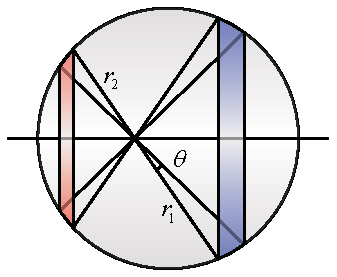
\includegraphics[width=5.2cm]{./figures/SphF1.pdf}
\caption{圆环的引力场} \label{SphF_fig1}
\end{figure}

由问题的对称性, 所求引力场由 $P$ 指向 $O$. 若我们将圆环划分为许多小段, 每小段质量为 $m_i$, 则 $m_i$ 在点 $P$ 产生的引力场在 $PO$ 方向的分量为
\begin{equation}
g_i = \frac{Gm_i}{r^2}\cos\theta
\end{equation}
所以总引力场大小等于
\begin{equation}\label{SphF_eq2}
g = \sum_i g_i = \frac{GM}{r^2}\cos\theta
\end{equation}

\subsection{均匀球壳内的引力场(几何法)}

\begin{figure}[ht]
\centering
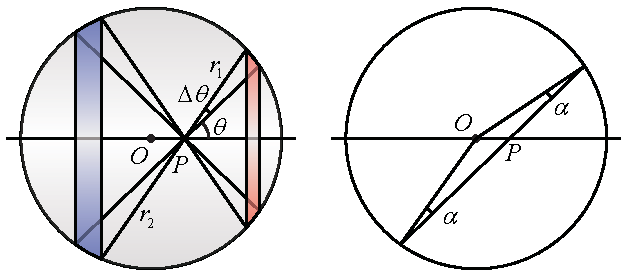
\includegraphics[width=10cm]{./figures/SphF2.pdf}
\caption{几何法} \label{SphF_fig2}
\end{figure}

我们现在来证明一个质量面密度为 $\sigma$ 的均匀球壳在其内部一点 $P$ 产生的引力场为零. 如\autoref{SphF_fig2}, 令球心为 $O$, 并过 $OP$ 作一个轴, 这样球面上任意一点都对应一个张角 $\theta$. 根据不同的 $\theta$ ($0 < \theta < \pi/2$)可将球壳划分为许多对细圆环, 每个圆环对应一个 $\Delta\theta$. 当 $\Delta\theta\to 0$ 时, 如果能证明任意一对细圆环在 $P$ 点产生的引力场都能互相抵消, 那么球壳对 $P$ 点的总引力场就为零.

我们先要求出两个圆环的面积, 以左图中右边的圆环为例, 圆环的周长为 $2\pi r_1\sin\theta$, 当 $\Delta\theta\to 0$ 时, 圆环的宽度为 $r_1\Delta\theta/\cos\alpha$ ($\alpha$ 的定义见右图), 所以圆环的面积等于周长乘以宽度, 再乘以面密度 $\sigma$ 得到右圆环的质量
\begin{equation}
M_1 = 2\pi r_1^2 \sigma \Delta\theta\sin\theta /\cos\alpha
\end{equation}
同理, 左圆环的质量为
\begin{equation}
M_2 = 2\pi r_2^2 \sigma \Delta\theta\sin\theta /\cos\alpha
\end{equation}
将 $M_1, r_1$ 和 $M_2, r_2$ 分别代入\autoref{SphF_eq2} 可得 $g_1 = g_2$ 即两圆环在 $P$ 点产生的引力场大小相等, 方向相反, 总引力场为零. 证毕.

\subsection{均匀球壳内的引力场(积分法)}
下面我们通过直接积分的方法求解球壳内外的引力场分布. 注意这个积分较为繁琐, 不感兴趣的读者可以直接看结论.

\begin{figure}[ht]
\centering
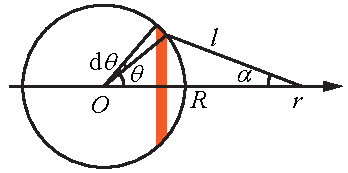
\includegraphics[width=6.2cm]{./figures/SphF3.pdf}
\caption{积分法} \label{SphF_fig3}
\end{figure}

如\autoref{SphF_fig3}, 令场点离原点 $O$ 的距离为 $r$ (虽然图中 $r > R$, 但 $r < R$ 时以下推导同样成立). 和以上推导类似, 图中圆环的面积为周长乘以宽度, 质量为
\begin{equation}
\dd{M} = 2\pi R\sin\theta\cdot R\dd{\theta}\cdot \sigma
= 2\pi R^2 \sigma \sin\theta \dd{\theta}
\end{equation}
圆环在场点产生的引力场为
\begin{equation}\label{SphF_eq6}
\dd{g} = \frac{G\dd{M}}{l^2}\cos\alpha
\end{equation}
其中 $\cos\alpha = (r - R\cos\theta)/l$. 由余弦定理, $l = R^2 + r^2 - 2Rr\cos\theta$. 将 $\dd{M}$, $\cos\alpha$ 和 $l$ 代入\autoref{SphF_eq6} 再对 $\theta$ 作定积分得
\begin{equation}\label{SphF_eq7}
g = 2\pi R^2 G\sigma \int_0^\pi \frac{(r - R\cos\theta)\sin\theta}{(R^2 + r^2 - 2Rr\cos\theta)^{3/2}} \dd{\theta}
\end{equation}
将上式中的定积分记为 $I$, 使用第一类换元积分法, 令 $x = \cos\theta$, 得
\begin{equation}\ali{
I &= \int_{-1}^1 \frac{r - Rx}{(R^2 + r^2 - 2Rrx)^{3/2}} \dd{x}\\
&= \frac{1}{2r} \int_{-1}^1 \frac{(r^2 - R^2) + (R^2 + r^2 - 2Rrx)}{(R^2 + r^2 - 2Rrx)^{3/2}} \dd{x}\\
&= \frac{r^2 - R^2}{2r} \int_{-1}^1 \frac{1}{(R^2 + r^2 - 2Rrx)^{3/2}} \dd{x} + 
\frac{R^2}{2r} \int_{-1}^1 \frac{1}{\sqrt{R^2 + r^2 - 2Rrx}} \dd{x}
}\end{equation}
这两个积分可以由“积分表\upref{ITable}” 中的\autoref{ITable_eq2} 结合\autoref{ITable_eq1} 得到.
\begin{equation}\label{SphF_eq9}
\ali{
I &= \frac{r^2 - R^2}{2r^2 R} \qty(\frac{1}{\abs{r - R}} - \frac{1}{\abs{r + R}}) - \frac{1}{2r^2 R} \qty(\abs{r - R} - \abs{r + R})\\
&= \leftgroup{&2/r^2 &\quad &(r > R)\\ &0 && (r < R)}
}\end{equation}
令球壳的质量为 $M = 4\pi R^2\sigma$, 则将\autoref{SphF_eq9} 代入\autoref{SphF_eq7} 得引力场为
\begin{equation}
g = \leftgroup{&GM/r^2 &\quad &(r > R)\\ &0 && (r < R)}
\end{equation}
当 $r < R$ 时, 引力场为零, 与上面的“几何法” 结论一致, 当 $r > R$ 时, 我们发现引力场等同于球心处质量相同的质点产生的引力场.

\subsection{球体的引力场}
我们最后来考虑一个体密度为 $\rho(r)$ 的球体在球内外产生的引力场. 我们可以把球体划分成任意多个质量均匀的薄球壳, 若 $r > R$, 每个球壳在场点的引力场都等效于球心处等质量的质点产生的引力场, 所以球体的引力场仍然等于球心处等质量质点产生的引力场.

当 $r < R$ 时, 所有半径大于 $r$ 的球壳在场点的场强为零, 而所有半径小于 $r$ 的球壳在场点的引力场等于球心处等质量的质点产生的引力场. 综上, 有
\begin{equation}
g = \leftgroup{&GM_0(r)/r^2 &\quad &(r > R)\\ &0 && (r < R)}
\end{equation}
其中
\begin{equation}
M_0(r) = \int_0^r 4\pi r^2 \rho(r) \dd{r}
\end{equation}

% 未完成: 例:均匀球体的势函数分布